\documentclass{beamer}
\usepackage[utf8]{inputenc}
\usepackage{graphicx}
\usepackage{xcolor}
\usepackage{forest}
\usepackage{amsmath}
\usepackage{algorithm}
\usepackage{algpseudocode}
\usepackage{tikz}
\usepackage[style=verbose,citetracker=false,backend=biber]{biblatex} 
\addbibresource{sample.bib}

\usetheme{Copenhagen}
\useoutertheme{smoothtree} % <<<<<<<<<<<<<<<<<<
\setbeamertemplate{footline}{
  \leavevmode%
  \hbox{%
    \begin{beamercolorbox}[wd=0.33\paperwidth,ht=2.5ex,dp=1ex,center]{author in head/foot}%
      \usebeamerfont{author in head/foot}A. Herrero
    \end{beamercolorbox}%
    \begin{beamercolorbox}[wd=0.34\paperwidth,ht=2.5ex,dp=1ex,center]{title in head/foot}%
      \usebeamerfont{title in head/foot}Project ADS
    \end{beamercolorbox}%
    \begin{beamercolorbox}[wd=0.33\paperwidth,ht=2.5ex,dp=1ex,right]{date in head/foot}%
      \usebeamerfont{date in head/foot}\insertframenumber{} / \inserttotalframenumber\hspace{1em}
    \end{beamercolorbox}%
  }
}

\definecolor{quack}{RGB}{75,0,130}
\usecolortheme[named=quack]{structure}

\begin{document}

\AtBeginSubsection[]
{
  \begin{frame}<beamer>
  \frametitle{Outline}
  \tableofcontents[currentsection,currentsubsection]
  \end{frame}
}

%------------------------------------------------------------
%This block of code defines the information to appear in the
%Title page
% Title page configuration
\title[Breaking the Binary Search Tree: A Tragicomic Tale of Random Insertions and Deletions]{
    Breaking the Binary Search Tree: A Tragicomic Tale of Random Insertions and Deletions
}

\author[A.Herrero]{
  \begin{minipage}[t]{0.5\textwidth}
    \raggedright
    \small \textit{Author:} \\
    \textbf{Alex Herrero} \\
    \vspace{1cm} % Adjust vertical spacing between author names and professor names
  \end{minipage}%
  \begin{minipage}[t]{0.5\textwidth}
    \raggedleft
    \small \textit{Professors:} \\
    \textbf{Conrado Martínez} \\
    \textbf{Amalia Duch} \\
    \textbf{Salvador Roura} \\
  \end{minipage} \\
  \vspace{1cm} % Adjust space to control the position of the logo
  \begin{center}
    
\includegraphics[scale=0.15]{logo-upc.png}
  \end{center}
}

% Remove navigation symbols
\beamertemplatenavigationsymbolsempty

%End of title page configuration block
%------------------------------------------------------------



%------------------------------------------------------------
\AtBeginSection[ ]
{
    \begin{frame}
        \tableofcontents[currentsection]
    \end{frame}
}
%------------------------------------------------------------

%The next statement creates the title page.
\frame{\titlepage}

\begin{frame}
\frametitle{Acknowledgment}
Special thanks to Conrado Martínez. 
His $\Theta(A(2^{n!}, m\log m))$\footnote{Where $A$ is the Ackermann function. Not the inverse!!} 
wisdom and advice  have been helpful throughout this project.
\end{frame}

%---------------------------------------------------------
%This block of code is for the table of contents after
%the title page
\begin{frame}
    \frametitle{Table of Contents}
    \tableofcontents
\end{frame}
%---------------------------------------------------------

\section{Introduction to BSTs}
\begin{frame}{Introduction to BSTs}
    
\begin{columns}[c]
% Column 1
    \begin{column}{0.5\textwidth}
     \begin{itemize}
         \item He introduced the concept of BST on his paper: ~\fullcite{hibbard1962}.
     \end{itemize}
    \end{column}
% Column 2    
    \begin{column}{0.5\textwidth}
        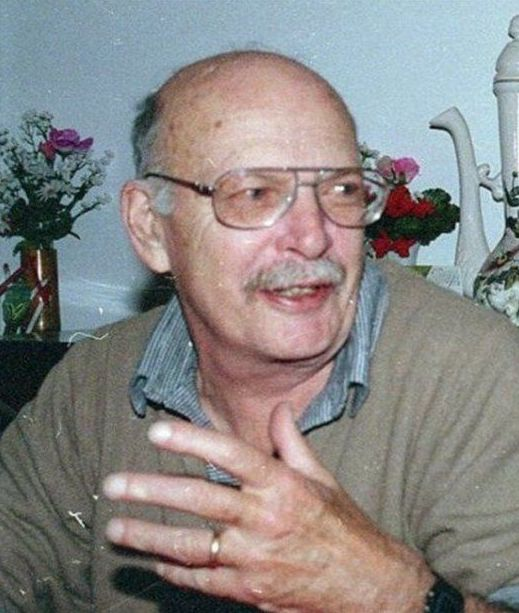
\includegraphics[width=\textwidth]{hibbard.jpg}
        \begin{center}
            Thomas Hibbard (1929-2016)
        \end{center}
    \end{column}
    
\end{columns}
\end{frame}

\begin{frame}
    \begin{itemize}
        \item He introduced not only the concept of binary search trees (BSTs), but also the idea of randomness in BSTs.
            \pause
        \item Well-known concepts and algorithms for every computer scientist.
            \pause
        \item We will take a look to Hibbard's deletion algorithm.
    \end{itemize}
\end{frame}

\begin{frame}{Leaf case}
    \begin{center}
        % Overlay 1: Original Tree
        \only<1>{
            \begin{forest}
                for tree={circle,draw, s sep=10mm}
                [8
                    [3
                        [1]
                        [6
                            [4]
                            [7]
                        ]
                    ]
                    [10
                        [,phantom]
                        [14
                            [13]
                            [,phantom]
                        ]
                    ]
                ]
            \end{forest}
        }

        % Overlay 2: Highlighted leaf
        \only<2>{
            \begin{forest}
                for tree={circle,draw, s sep=10mm}
                [8
                    [3
                        [1]
                        [6
                            [4]
                            [7, color=red]
                        ]
                    ]
                    [10
                        [,phantom]
                        [14
                            [13]
                            [,phantom]
                        ]
                    ]
                ]
            \end{forest}
        }

        % Overlay 3: Leaf removed
        \only<3>{
            \begin{forest}
                for tree={circle,draw, s sep=10mm}
                [8
                    [3
                        [1]
                        [6
                            [4]
                            [,phantom]
                        ]
                    ]
                    [10
                        [,phantom]
                        [14
                            [13]
                            [,phantom]
                        ]
                    ]
                ]
            \end{forest}
        }
    \end{center}
\end{frame}

\begin{frame}{Only one subtree case}
    \begin{center}
        % Overlay 1: Original Tree
        \only<1>{
            \begin{forest}
                for tree={circle,draw, s sep=10mm}
                [8
                    [3
                        [1]
                        [6
                            [4]
                            [7]
                        ]
                    ]
                    [10
                        [,phantom]
                        [14
                            [13]
                            [,phantom]
                        ]
                    ]
                ]
            \end{forest}
        }

        % Overlay 2: Highlighted leaf
        \only<2>{
            \begin{forest}
                for tree={circle,draw, s sep=10mm}
                [8
                    [3
                        [1]
                        [6
                            [4]
                            [7]
                        ]
                    ]
                    [10
                        [,phantom]
                        [14, color=red
                            [13]
                            [,phantom]
                        ]
                    ]
                ]
            \end{forest}
        }

        % Overlay 3: Leaf removed
        \only<3>{
            \begin{forest}
                for tree={circle,draw, s sep=10mm}
                [8
                    [3
                        [1]
                        [6
                            [4]
                            [7]
                        ]
                    ]
                    [10
                        [,phantom]
                        [13]
                    ]
                ]
            \end{forest}
        }
    \end{center}
\end{frame}


\begin{frame}{Two subtree case}
    \begin{center}
        % Overlay 1: Original Tree
        \only<1>{
            \begin{forest}
                for tree={circle,draw, s sep=10mm}
                [8
                    [3
                        [1]
                        [6
                            [4]
                            [7]
                        ]
                    ]
                    [10
                        [,phantom]
                        [14
                            [13]
                            [,phantom]
                        ]
                    ]
                ]
            \end{forest}
        }

        % Overlay 2: Highlighted leaf
        \only<2>{
            \begin{forest}
                for tree={circle,draw, s sep=10mm}
                [8
                    [3, color=red
                        [1]
                        [6
                            [4]
                            [7]
                        ]
                    ]
                    [10
                        [,phantom]
                        [14
                            [13]
                            [,phantom]
                        ]
                    ]
                ]
            \end{forest}
        }

        % Overlay 3: Leaf removed
        \only<3>{
            \begin{forest}
                for tree={circle,draw, s sep=10mm}
                [8
                    [3, color=red
                        [1]
                        [6
                            [4, color=green]
                            [7]
                        ]
                    ]
                    [10
                        [,phantom]
                        [14
                            [13]
                            [,phantom]
                        ]
                    ]
                ]
            \end{forest}
        }
        \only<4>{
            \begin{forest}
                for tree={circle,draw, s sep=10mm}
                [8
                    [4, color=green
                        [1]
                        [6
                            [3, color=red]
                            [7]
                        ]
                    ]
                    [10
                        [,phantom]
                        [14
                            [13]
                            [,phantom]
                        ]
                    ]
                ]
            \end{forest}
        }
        \only<5>{
            \begin{forest}
                for tree={circle,draw, s sep=10mm}
                [8
                    [4, color=green
                        [1]
                        [6
                            [,phantom]
                            [7]
                        ]
                    ]
                    [10
                        [,phantom]
                        [14
                            [13]
                            [,phantom]
                        ]
                    ]
                ]
            \end{forest}
        }
    \end{center}
\end{frame}

\begin{frame}
    \footnotesize
    \begin{algorithmic}
        \Function{delete}{$T$, $x$}
        \If{$T.val < x$}
        \State $T.right \gets$ \Call{delete}{$T.right$, $x$}
        \ElsIf{$T.val > x$}
        \State $T.left \gets$ \Call{delete}{$T.left$, $x$}
        \Else
        \If{$T.right = \text{null}$}
        \State \Return $T.left$
        \Else
        \State $T.val \gets$ \Call{minValue}{$T.right$}
        \State $T.right \gets$ \Call{delete}{$T.right$, $T.val$}
        \EndIf
        \EndIf
        \State \Return $T$
        \EndFunction
    \end{algorithmic}
\end{frame}

\begin{frame}
    Hibbard’s paper was remarkable in that it contained one of the first formal theorems about algorithms:
    \pause
    \begin{block}{Hibbard's Theorem (1962)}
        If $n + 1$ items are inserted into an initially empty binary tree, in random order, and if one of those items (selected at random) is deleted, the probability that the resulting binary tree has a given shape is the same as the probability that this tree shape would be obtained by inserting $n$ items into an initially empty tree, in random order.
    \end{block}
    \pause
    It is reasonable to think that Hibbard's deletion algorithm preserves the randomness of BSTs...
    \pause
    And it was believed for more than $10$ years!
\end{frame}

\begin{frame}
    \begin{block}{Donald Knuth}
        The $I^*D_r$ property might seem to be all that one needs to guarantee insensitivity to \textit{any} number of deletions, when they are intermixed with insertions in any order. At least, many people (including the present author when writing the first edition of \textit{The Art of Computer Programming Vol:3}) believed this\footcite{knuth1977deletions}.
    \end{block}
\end{frame}

\section{Paradoxical result}

\begin{frame}
    
\begin{columns}[c]
% Column 1
    \begin{column}{0.5\textwidth}
     \begin{itemize}
         \item It was believed for more than a decade that Hibbard's algorithm preserved randomness on BSTs
             \pause
         \item $1975$: \cite{knott1975deletion}
     \end{itemize}
    \end{column}
% Column 2    
    \begin{column}{0.5\textwidth}
        \begin{center}
            \begin{block}{Knott Paradox}
                Although Hibbard’s theorem establishes that n+1 random insertions
                followed by a random deletion produce a tree whose shape has the distribution of n random insertions, it does not follow that a
                subsequent random insertion yields a tree whose shape has the distribution of n+1 random insertions
            \end{block}
        \end{center}
    \end{column}
    
\end{columns}
\end{frame}

\begin{frame}
    We will follow the explanaition from \cite{jonassen1978trivial} for a BST of size $n = 3$
\end{frame}

\begin{frame}{All BSTs for $x < y < z$}
    \begin{center}
        \begin{tabular}{cccccc}
            $(x, y, z)$ &
            $(x, z, y)$ &
            $(y, x, z) = (y, z, x)$ &
            $(z, x, y)$ &
            $(z, y, x)$ \\
            \begin{tikzpicture}[level distance=0.6cm,sibling distance=0.6cm]
                \node {x}
                    child[missing]
                    child {node {y}
                        child[missing]
                    child {node {z}}};
            \end{tikzpicture}
                                           &
                                           \begin{tikzpicture}[level distance=0.6cm,sibling distance=0.6cm]
                                               \node {x}
                                                   child[missing]
                                                   child {node {z}
                                                       child {node {y}}
                                                   child[missing]};
                                           \end{tikzpicture}
                                           &
                                           \begin{tikzpicture}[level distance=0.6cm,sibling distance=0.8cm]
                                               \node {y}
                                                   child {node {x}}
                                                   child {node {z}};
                                           \end{tikzpicture}
                                           &
                                           \begin{tikzpicture}[level distance=0.6cm,sibling distance=0.6cm]
                                               \node {z}
                                                   child {node {x}
                                                       child[missing]
                                                   child {node {y}}}
                                                   child[missing];
                                           \end{tikzpicture}
                                           &
                                           \begin{tikzpicture}[level distance=0.6cm,sibling distance=0.6cm]
                                               \node {z}
                                                   child {node {y}
                                                       child {node {x}}
                                                   child[missing]}
                                                   child[missing];
                                           \end{tikzpicture}
                                           \\
            $RR$ & 
            $RL$ &
            $B$ &
            $LR$ &
            $LL$ &
        \end{tabular}
    \end{center}
\end{frame}

\begin{frame}
    \begin{center}
        \begin{tabular}{||c c c c||} 
            \hline
            Permutation& Delete $x$& Delete $y$ & Delete $z$ \\ [0.5ex] 
            \hline\hline
            $(x,y,z)$ & $R$ & $R$ & $R$ \\ 
            \hline
            $(x,z,y)$ & $R$ & $R$ & $R$ \\ 
            \hline
            $(y,z,x) = (y,x,z)$ & $R$ & $L$ & $L$\\ 
            \hline
            $(z,x,y)$ & $L$ & $L$ & $R$\\ 
            \hline
            $(z,y,x)$ & $L$ & $L$ & $L$ \\ 
            \hline
        \end{tabular}
    \end{center}
    \begin{center}
        \pause
        $$
        \mathbb{P}[L] = \frac{9}{18} = \frac{1}{2}
        $$
        $$
        \mathbb{P}[R] = \frac{9}{18} = \frac{1}{2}
        $$
    \end{center}
\end{frame}

\begin{frame}
    Now another random insertion $w$ comes to the BST. Then we have four possible cases:
    \begin{itemize}
        \pause
        \item $w < x < y < z$
        \pause
        \item $x < w < y < z$
        \pause
        \item $x < y < w < z$
        \pause
        \item $x < y < z < w$
    \end{itemize}
    \pause
    $18$ previous cases and $4$ possibilities for $w$ give us a total of $72$ cases.
\end{frame}

\begin{frame}{Inserting $w$}
    $w < x < y < z$
    \begin{center}
        \begin{tabular}{||c c c c||} 
            \hline
            Permutation& Delete $x$& Delete $y$ & Delete $z$ \\ [0.5ex] 
            \hline\hline
            $(x,y,z)$ & $B$ & $B$ & $B$ \\ 
            \hline
            $(x,z,y)$ & $B$ & $B$ & $B$ \\ 
            \hline
            $(y,z,x) = (y,x,z)$ & $B$ & $LL$ & $LL$\\ 
            \hline
            $(z,x,y)$ & $LL$ & $LL$ & $B$\\ 
            \hline
            $(z,y,x)$ & $LL$ & $LL$ & $LL$ \\ 
            \hline
        \end{tabular}
    \end{center}
\end{frame}

\begin{frame}{Inserting $w$}
    $x < w < y < z$
    \begin{center}
        \begin{tabular}{||c c c c||} 
            \hline
            Permutation& Delete $x$& Delete $y$ & Delete $z$ \\ [0.5ex] 
            \hline\hline
            $(x,y,z)$ & $B$ & $RL$ & $RL$ \\ 
            \hline
            $(x,z,y)$ & $B$ & $RL$ & $RL$ \\ 
            \hline
            $(y,z,x) = (y,x,z)$ & $B$ & $LR$ & $LR$\\ 
            \hline
            $(z,x,y)$ & $LL$ & $LR$ & $RL$\\ 
            \hline
            $(z,y,x)$ & $LL$ & $LR$ & $LR$ \\ 
            \hline
        \end{tabular}
    \end{center}
\end{frame}

\begin{frame}{Inserting $w$}
    $x < y < w < z$
    \begin{center}
        \begin{tabular}{||c c c c||} 
            \hline
            Permutation& Delete $x$& Delete $y$ & Delete $z$ \\ [0.5ex] 
            \hline\hline
            $(x,y,z)$ & $RL$ & $RL$ & $RR$ \\ 
            \hline
            $(x,z,y)$ & $RL$ & $RL$ & $RR$ \\  
            \hline
            $(y,z,x) = (y,x,z)$ & $RL$ & $LR$ & $B$\\ 
            \hline
            $(z,x,y)$ & $LR$ & $LR$ & $RR$\\ 
            \hline
            $(z,y,x)$ & $LR$ & $LR$ & $B$ \\ 
            \hline
        \end{tabular}
    \end{center}
\end{frame}

\begin{frame}{Inserting $w$}
    $x < y < z < w$
    \begin{center}
        \begin{tabular}{||c c c c||} 
            \hline
            Permutation& Delete $x$& Delete $y$ & Delete $z$ \\ [0.5ex] 
            \hline\hline
            $(x,y,z)$ & $RR$ & $RR$ & $RR$ \\ 
            \hline
            $(x,z,y)$ & $RR$ & $RR$ & $RR$ \\  
            \hline
            $(y,z,x) = (y,x,z)$ & $RR$ & $B$ & $B$\\ 
            \hline
            $(z,x,y)$ & $B$ & $B$ & $RR$\\ 
            \hline
            $(z,y,x)$ & $B$ & $B$ & $B$ \\ 
            \hline
        \end{tabular}
    \end{center}
\end{frame}

\begin{frame}{Probabilities}
    \begin{align*}
        \mathbb{P}[LL] &= \frac{11}{72} & \quad \mathbb{P}[LR] &= \frac{13}{72} \\
        \mathbb{P}[RL] &= \frac{11}{72} & \quad \mathbb{P}[RR] &= \frac{12}{72}
    \end{align*}
        $$
        \mathbb{P}[B] = \frac{25}{72}
        $$
        Know another random deletion comes. Let us analyze the probability of having and $L$ shape:
    \pause
    \begin{block}{Probability $L$ Shape}
        The probability of having an $L$ shape after a random deletion is: $\mathbb{P}[L] = \mathbb{P}[LL] + \frac{2}{3}  \mathbb{P}[LR] + \frac{2}{3} \mathbb{P}[B] = \frac{11}{72} + \frac{2}{3} \cdot \frac{13}{72} + \frac{2}{3} \cdot \frac{25}{72} = \frac{109}{216} > \frac{1}{2}$!!
    \end{block}
    \pause
    Actually it makes sense! 
\end{frame}

\begin{frame}
    \begin{center}
        \only<1>{
            \begin{forest}
                for tree={circle,draw, s sep=10mm}
                [25
                    [20
                        [10
                            [5]
                            [12]
                        ]
                        [22]
                    ]
                    [36
                        [30
                            [28]
                            [,phantom]
                        ]
                        [40
                            [38]
                            [48]
                        ]
                    ]
                ]
            \end{forest}
        }

        \only<2>{
            \begin{forest}
                for tree={circle,draw, s sep=10mm}
                [25, color=red
                    [20
                        [10
                            [5]
                            [12]
                        ]
                        [22]
                    ]
                    [36
                        [30
                            [28]
                            [,phantom]
                        ]
                        [40
                            [38]
                            [48]
                        ]
                    ]
                ]
            \end{forest}
        }

        \only<3>{
            \begin{forest}
                for tree={circle,draw, s sep=10mm}
                [25,color=red
                    [20
                        [10
                            [5]
                            [12]
                        ]
                        [22]
                    ]
                    [36
                        [30
                            [28,color=green]
                            [,phantom]
                        ]
                        [40
                            [38]
                            [48]
                        ]
                    ]
                ]
            \end{forest}
        }

        \only<4>{
            \begin{forest}
                for tree={circle,draw, s sep=10mm}
                [28
                    [20
                        [10
                            [5]
                            [12]
                        ]
                        [22]
                    ]
                    [36
                        [30]
                        [40
                            [38]
                            [48]
                        ]
                    ]
                ]
            \end{forest}
            \pause

            Did we change the probability of inserting a random element into one subtree? Somehow, yes...
        }
    \end{center}
\end{frame}

\begin{frame}
    \begin{block}{Donald Knuth}
        The shape of the tree is random after deletions, but the relative distribution of values in a given tree shape may change, and it turns out that the first random insertion, after a deletion actually destroys the randomness property on shapes. This startling fact, first observed by Gary Knott in 1972, must be seen to be believed\footcite{knuth1998art}
    \end{block}
\end{frame}

\begin{frame}
    Knott was the first to notice that Hibbard's generalization was wrong. 
    \pause

    In his thesis he also gave some empirical data summarizing the results of simulation experiments, where BSTs randomly constructed by $I^n(ID)^m$. Leading to the following conjecture:
    \begin{block}{Knott's conjecture}
        Empirical evidence suggests strongly that the path length tends to decrease after repeated deletions and insertions, so the
        departure from randomness seems to be in the right direction; a theoretical explanation for this behavior is still lacking\footcite{knuth1998art}
    \end{block}
\end{frame}

\section{Experimental Results}

\begin{frame}
    \begin{columns}[c]
        % Column 1
        \begin{column}{0.5\textwidth}
            \begin{itemize}
                \item ~\fullcite{eppinger1983}.
                \item A landmark in experimental algorithmic literature
            \end{itemize}
        \end{column}
        % Column 2    
        \begin{column}{0.5\textwidth}
            
\includegraphics[width=\textwidth]{eppinger.jpg}
            \begin{center}
                Jeffrey Eppinger (1960)
            \end{center}
        \end{column}
    \end{columns}
\end{frame}

\begin{frame}
    Recall:
    \begin{itemize}
        \item The expected number of comparisons used when searching for an element in a binary tree is proportional to the tree's path length
            \pause
        \item $IPL = \sum\limits_{v \in V(T)} d(root, v)$
            \pause
        \item For a random tree containing $n$ nodes the expected IPL is denoted as $I_n$. The expected number of comparisons in a successful search is denoted as $C_n$
        \item Knuth \footcite{knuth1998art} give the expected number of comparisons in a successful search, $C_n$, as $2(1 + \frac{1}{n})H_n - 3$
        \item By the relation $I_n = n(C_n - 1)$ one obtains the approximation $1.386n \log n - 2.846n$
            \pause
        \item A distribution of trees is said to be "better than random" when the expected IPL is less than $I_n$.
    \end{itemize}
\end{frame}

\begin{frame}
    \begin{itemize}
        \item Large samples of random BSTs of various sizes
        \item Based on Knott's experiments, extended with more insertions and deletions (a quadratic number in particular)
    \end{itemize}
\end{frame}

\begin{frame}[plain]
    \begin{center}
        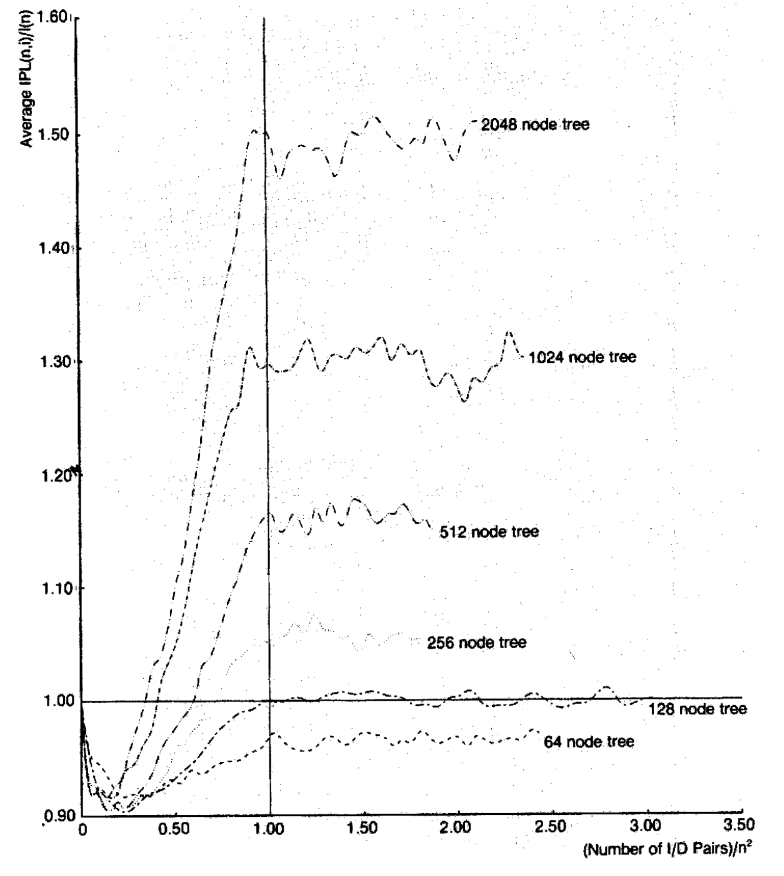
\includegraphics[width=\paperwidth,height=\paperheight,keepaspectratio]{plotEppinger.png}
    \end{center}
\end{frame}

\begin{frame}
    \begin{itemize}
        \item Hibbard's algorithm is asymmetric (always choose right subtree)
            \pause
        \item A symmetric version of this algorithm was trivially implemented by Eppinger
    \end{itemize}
\end{frame}

\begin{frame}
    \footnotesize
    \begin{algorithmic}
        \Function{Symmetric delete}{$T$, $x$}
        \If{$T.val < x$}
        \State $T.right \gets$ \Call{Symmetric delete}{$T.right$, $x$}
        \ElsIf{$T.val > x$}
        \State $T.left \gets$ \Call{Symmetric delete}{$T.left$, $x$}
        \Else
        \If{$T.right = \text{null}$}
        \State \Return $T.left$
        \Else
        \If{\Call{flipCoin} $= Head$}
        \State $T.val \gets$ \Call{minValue}{$T.right$}
        \State $T.right \gets$ \Call{Symmetric delete}{$T.right$, $T.val$}
        \Else
        \State $T.val \gets$ \Call{maxValue}{$T.left$}
        \State $T.left \gets$ \Call{Symmetric delete}{$T.left$, $T.val$}
        \EndIf
        \EndIf
        \EndIf
        \State \Return $T$
        \EndFunction
    \end{algorithmic}
\end{frame}

\begin{frame}[plain]
    \begin{center}
        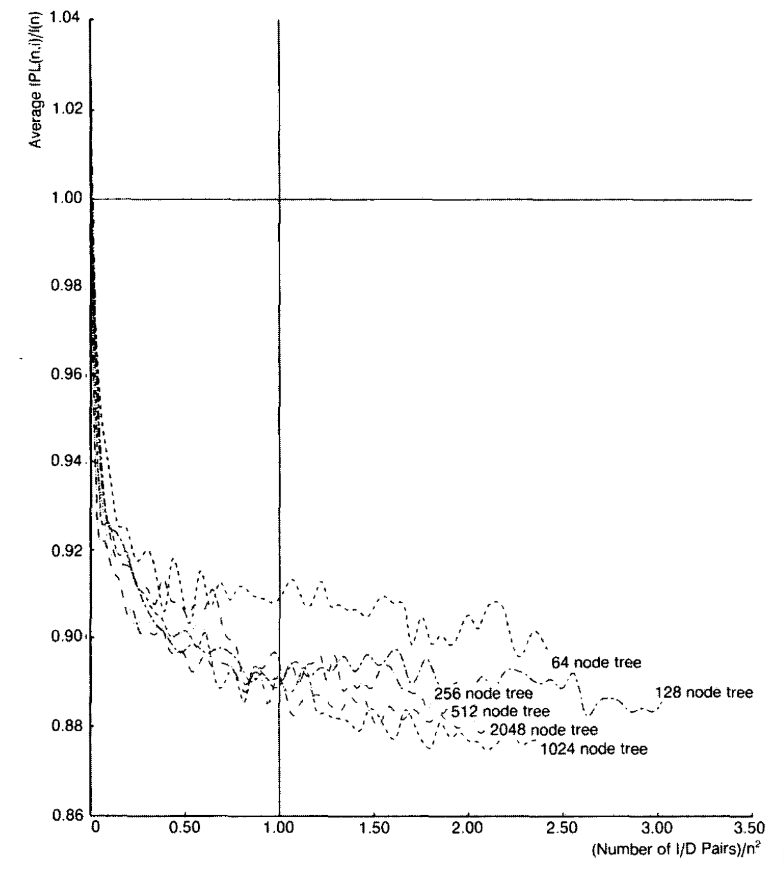
\includegraphics[width=\paperwidth,height=\paperheight,keepaspectratio]{plotEppingerSym.png}
    \end{center}
\end{frame}

\begin{frame}{Comparison of Deletions}
    \centering
    \begin{minipage}{0.48\textwidth}
        \centering
        \textbf{Asymmetric Deletions}

        \resizebox{\textwidth}{!}{%
            \begin{tabular}{|c|c|c|c|}
                \hline
                $n$ & Samples & $\overline{IPL}_n$ & Variance \\
                \hline
                64   & 6000  & 0.97 & 0.01652 \\
                128  & 6800  & 1.00 & 0.01340 \\
                256  & 2300  & 1.06 & 0.00985 \\
                512  & 1200  & 1.16 & 0.00970 \\
                1024 & 750   & 1.30 & 0.01013 \\
                2048 & 5340  & 1.49 & 0.00771 \\
                \hline
            \end{tabular}
        }
    \end{minipage}
    \hfill
    \begin{minipage}{0.48\textwidth}
        \centering
        \textbf{Symmetric Deletions}

        \resizebox{\textwidth}{!}{%
            \begin{tabular}{|c|c|c|c|}
                \hline
                $n$ & Samples & $\overline{IPL}_n$ & Variance \\
                \hline
                64   & 6000  & 0.905 & 0.01654 \\
                128  & 6800  & 0.890 & 0.00916 \\
                256  & 2300  & 0.888 & 0.00615 \\
                512  & 1200  & 0.890 & 0.00347 \\
                1024 & 750   & 0.881 & 0.00235 \\
                2048 & 5340  & 0.883 & 0.00269 \\
                \hline
            \end{tabular}
        }
    \end{minipage}
    Data obtained after a quadratic number of insertions/deletions.
\end{frame}

\begin{frame}[plain]
    \begin{center}
        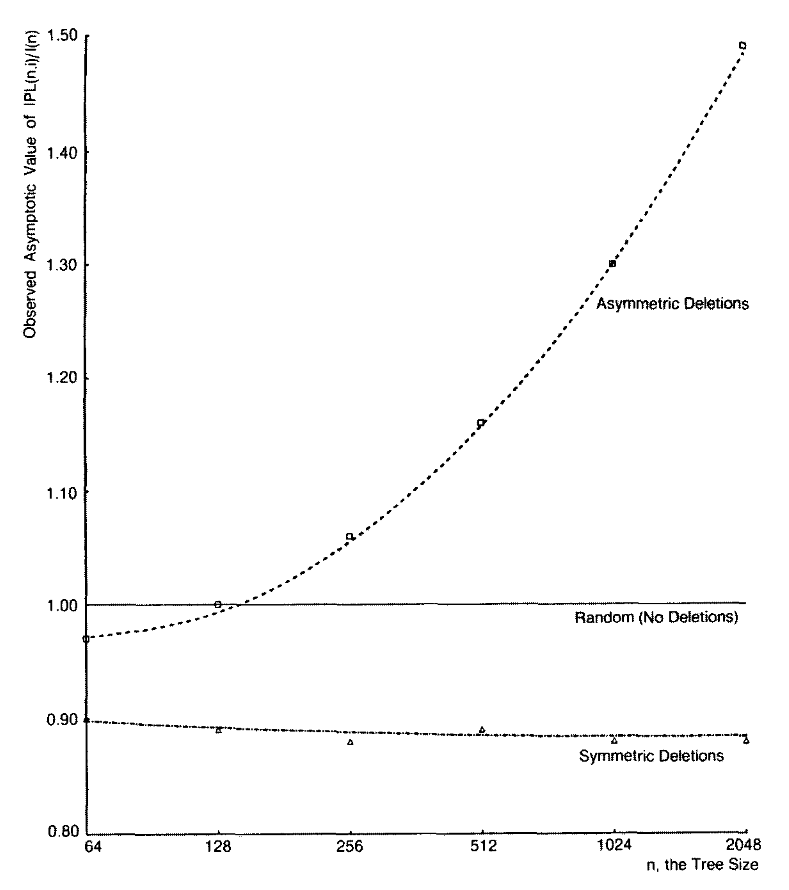
\includegraphics[width=\paperwidth,height=\paperheight,keepaspectratio]{asymp.png}
    \end{center}
\end{frame}



\begin{frame}{Asymmetric Deletion}
    A least-square multiple regression weighted by the inverse of the variance yields to the following approximation:
    \pause
    $$
    \lim_{i \to \infty} \frac{\overline{IPL_{n,i}}}{I_n} \approx 0.0202 \log^2 n - 0.241 \log n + 1.69
    $$

    Substituting $I_n \approx 1.386n \log n - 2.846n$ we obtain:
    \pause

    $$
    \lim_{i \to \infty} \overline{IPL_{n,i}} \approx 0.0280n \log^3 n - 0.392n \log^2 n + 3.03n \log n - 4.81n
    $$

    \pause
    \begin{block}{Expected Internal Path Length}
        The expected IPL of a tree performing the asymmetric deletion algorithm is, experimentally, $\Theta(n \log^3 n)$
    \end{block}
\end{frame}

\begin{frame}{Symmetric Deletion}
    Symmetric Deletions?
    \pause
    $$
    \lim_{i \to \infty} \frac{\overline{IPL_{n,i}}}{I_n} \approx 0.88
    $$

    Or that
    $$
    \lim_{i \to \infty} \overline{IPL_{n,i}}\approx 1.22n \log n - 2.50n
    $$
    \pause
    \begin{block}{Expected Internal Path Length}
        The expected IPL of a tree performing the symmetric deletion algorithm is, experimentally, $\Theta(n \log n)$. Since the perfect tree has IPL $\Omega(n \log n)$ we know that, experimentally, this result is optimum!
    \end{block}
\end{frame}

\section{Theoretical Studies}

\begin{frame}{Explaining the Behaviour of Binary Search Trees Under Prolonged Updates: A Model and Simulations\footcite{culberson1989explaining}}
    \footnotesize
    \begin{block}{Abstract}
        In this paper we present an extensive study into the long-term behaviour of binary search trees subjected to updates using the usual deletion algorithms taught in introductory textbooks. We develop a model of the behaviour of such trees which \textbf{leads us to conjecture that the asymptotic average search path length is $\Theta(N^{0.5})$}. We present results of large simulations which strongly support this conjecture. \textbf{However, introducing a simple modification to ensure symmetry in the algorithms, the model predicts no such long-term deterioration. Simulations in fact indicate that asymptotically the average path length of such trees is less than the $1.386\ldots\log_2 N$ average path length of trees generated from random insertion sequences}
    \end{block}
\end{frame}

\begin{frame}{Analysis of the standard deletion algorithms in exact fit domain binary search trees\footcite{culberson1990analysis}}
    \begin{block}{Abstract}
        It is well known that the expected search time in an $N$ node binary search tree generated by a random sequence of insertions is $O(\log N)$. Little has been published about the asymptotic cost when insertions and deletions are made following the usual algorithms with no attempt to retain balance. \textbf{We show that after a sufficient number of updates, each consisting of choosing an element at random, removing it, and reinserting the same value, that the average search cost is $\Theta(N^{\frac{1}{2}})$}
    \end{block}
\end{frame}

\begin{frame}
    System of tagging a BST as follows:
    \begin{itemize}
        \item The smallest key in the tree receives a new tag whenever it is inserted
        \item Whenever a key is deleted, all the tags currently attached to it are moved to the next larger key, unless the deleted key is the largest, in which case its tags are discarded
    \end{itemize}
\end{frame}

\begin{frame}
    \begin{center}
        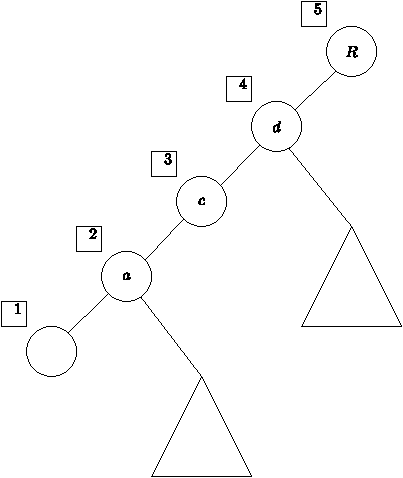
\includegraphics{tag.pdf}
    \end{center}
\end{frame}

\begin{frame}
    \pause
    \begin{alertblock}{Lemma 2}
        \textit{In an EFD the expected size of the interval containing the $j$th smallest key at the time it enters the interval is}
        $$
        E_j = \frac{2^{2j - 2}}{\binom{2j - 2}{j - 1}} - 1 \approx \sqrt{\pi j}
        $$
    \end{alertblock}
    \pause
    \begin{alertblock}{Lemma 3}
        \textit{The expected size of the $r$th subtree on an EFD after sufficiently many updates is $O(\sqrt{N})$ for all $r$}
    \end{alertblock}
    \pause
    \begin{alertblock}{Lemma 4}
        \textit{The expected number of nodes in the backbone of the EFD tree is $O(\sqrt{N})$ after sufficiently many updates}
    \end{alertblock}
\end{frame}
\begin{frame}
    \begin{alertblock}{Theorem 1}
        \textit{The IPL of the EFD tree is $\Theta(N^{3/2})$}
    \end{alertblock}
\end{frame}



\begin{frame}{Deletions that preserve randomness\footcite{knuth1977deletions}}
    \begin{block}{Abstract}
        This paper discusses dynamic properties of data structures under
        insertions and deletions. It is shown that, in certain circumstances,
        the result of $n$ random insertions and $m$ random deletions will be
        equivalent to $n-m$ random insertions, \textit{under various interpretations of
        the word \textit{random} and under various constraints on the order of insertions
    and deletions.}
    \end{block}
\end{frame}

\begin{frame}
    \begin{itemize}
        \item Abstract studies on deletion and insertion on any data structure
            \pause
        \item Generalization of Hibbard's theorem appears as \textit{one-step deletion insensitivity} abbreviated $I^* D_r$
            \pause
        \item Deletion insensitivity: $I^*D$, $I^*D^*$, $I^*DI^*$, $(I,D)^*$
            \pause
        \item \textit{Under various constraints on the order of insertions}: In particular three different types of insertions
        \item \textit{Under various constraints on the order of deletions}: In particular six different types of deletions
    \end{itemize}
\end{frame}


\begin{frame}{A trivial algorithm whose analysis isn't \footcite{jonassen1978trivial}}
    \begin{block}{Abstract}
        Very few theoretical results have been obtained to date about the behavior of information retrieval algorithms under random \textit{deletions}, as well as random insertions. The present paper offers a possible explanation for this dearth of results, by showing that one of the simplest such algorithms already requires a surprisingly intricate analysis. Even when \textbf{the data structure never contains more than three items at a time, it is shown that the performance of the standard tree search/insertion/deletion algorithm involves Bessel functions and the solution of bivariate integral equations}. A step-by-step expository analysis of this problem is given, and it is shown how the difficulties arise and can be surmounted.
    \end{block}
\end{frame}

\begin{frame}
    \begin{itemize}
        \item \url{https://doi.org/10.1016/0022-0000(78)90020-X}
            \pause
        \item "Random deletions do not always enhance the average path length; the pattern $IIIDIDIDI$ leads to a better average search time than does the same patter followed by $DI$
            \pause
        \item With Knuth's modification on Hibbard's algorithm (considering a special case as one separate case) they obtained the following:
    \end{itemize}
    \begin{block}{Last paragraph in Jonassen and Knuth article}
        (...) Since the values of $c_n$ in the unmodified algorithm are \textit{greater} than $1/3$, for $n \geq 1$, the average internal path length actually turns out to be worse when we use the ``improved'' algorithm. On the other hand, Knott's empirical data indicate that the modified algorithm does indeed lead to an improvement when the trees are larger.
    \end{block}
\end{frame}


\section{Final remarks}

\begin{frame}
    Do we know a deletion algorithm that preserve randomness?
    \pause
    \begin{itemize}
        \item \cite{martinez1998randomized}
        \item \cite{seidel1996randomized}
    \end{itemize}
\end{frame}

\begin{frame}
    Do you wanna know a little bit more about this Tragicomic Tale? Check:

    \cite{panny2010deletions}
\end{frame}

\section{References}
\printbibliography
\frame{\titlepage}


\end{document}
